%% Chapter 10 : Conclusion And Future Work

\section{Conclusion}
\
\
\
\
A complete application framework has been developed for the energy/power forecasting of SVPPs and WTPPs in MATLAB using its GUI feature.\\

A application for P-V and I-V curve generation for solar PV modules has been developed and successfully. It is able to generate the P-V and I-V curves under any temperature and irradiance condition; moreover shading analysis under presence/absence of Bypass Diodes can also be done. The accuracy of the application has been tested with five PV modules of different technologies as seen in chapter 2.\\

Solar energy estimation application has been developed. It is capable of simulating energy production of SVPPs with multiple PV technologies using instantaneous irradiance file or daily insolation file or clear sky solar flux model (modified by incorporating clearness index estimation using rainfall data). The application is tested with the Backbone plant data of year 2014 and compared with PVsyst software results. The results show improvements over PVsyst software as seen in cahapter 4.\\

Wind energy estimation application has been developed. It is capable of simulating energy production of WTPP's with multiple Wind Turbine technologies and their sub-types using the instantaneous wind speed file. Moreover, the application provides an interface for determining potential wind plant sites using minimum data through Weibull wind characteristics. The application is tested with a hypothetical wind plant data, the results show that the application runs smoothly without bugs as seen in chapter 5.\\

ARIMA forecasting application has been developed. It is capable of acquiring data through excel files of desired indices, model identification, model creation (AR, MA, ARIMA [Seasonal and Non-Seasonal]), Model Estimation and Fitness Check, and finally computing forecasts for desired number of observation points. During a single run it can handle one univariate time series and create/estimate multiple ARIMA models of different types from which the best model is selected for forecasting purposes. The application is tested with the weather data obtained from GSEC 1MW solar power plant in Gandhinagar, Gujarat and a forecast of the weather variables for one day in an interval of 4 hours with a temporal resolution of 15 minutes has been computed. The resultant forecast values are fed to the solar energy estimation app to generate the intra-day generation forecast. The results are very promising. \\

ANN forecasting application has been developed. It is capable of running in three different modes, moreover three different neural network architectures (fitnet, feed forward and cascaded feed forword) can be utilised with a wide variety of training functions. Multiple nets can be trained simultaneously to overcome the problem of randomly generated initial biases and weights. The application is rigorously tested with 11 months weather data of GSEC 1MW solar power plant in Gandhinagar, Gujarat
 which is used for training, and the trained nets are used to forecast the weather data for the remaining one month.The ouputs thus obtaind were fed to the solar energy estimation app to generate the forecasted energy of GSEC solar power plant for the untrained month. The results obtained are very promising as seen in chapter 8.\\

WRF software has been ported successfully to run on a 4 node Raspberry-Pi 2 cluster. Efficient bash scripts are developed to run every facet of the WRF software from the initialization data acquisition from a FTP server, to running the WPS pre-proceesing system and finally running the WRF system.The cluster and the bash scripts were tested by simulating a grid over the GSEC 1MW solar power plant, and simulations for the weather output files were carried out with a spatial resolution of 1Km and a temporal resolution of 15 minutes for entire month of June 2016. The required weather variables (irradiance, temperature and wind speed) for the desired location were extracted into excel files from the NETCDF output files produced by the WRF simulations using the WRF NETCDF visualiation and extraction application developed in MATLAB. These excel files were further post-processed and then fed as input to the solar energy estimation app to generate the forecasted energy of GSEC solar power plant for June 2016. The results thus obtained were compared with the June 2015 data of GSEC power plant as the latest data was unavailable. The results generated were promising.\\

An entire eco-system for performing generation forecasting for solar and wind power plants has been developed. The ANN and ARIMA are used for intra hour forecasting, ARIMA and WRF are used for intra-day forecasting, and WRF is used for day ahead forecasting. The application is running smoothly, but the only concern is lack of good quality historical data from the plant. Each sub module in the application structure is an independently functioning system dependent only on the required inputs. The energy estimation applications not only help in computing forecasted energy/power but also in computing energy/power outputs for plants under planning stage. The ANN and ARIMA apps make it easier to develop forecast models and the desired forecast very intuitively and in a short time. The automatized bash scripts for running the WRF software makes it very easy to use. Moreover, the successful implementation of the WRF software on a cluster of micro-computers is also achieved. As the entire application has a very functional and modular design, which enables for easy debugging and up-gradation of the application to suit the needs of varied end users.\\

\newpage

\section{Future Work}
\
\
\
\
For the future, we here at GERMI (Gujarat Energy Research And Management Institute) want to take this effort one step ahead i.e develop a Real-Time Forecasting System and manage the forecasting of a single megawatt size solar power plant. For this we will be developing our own Plant Database Management System with our own Data Logger as shown in Fig (\ref{figc10h1}).

\begin{figure}[H]
\centering
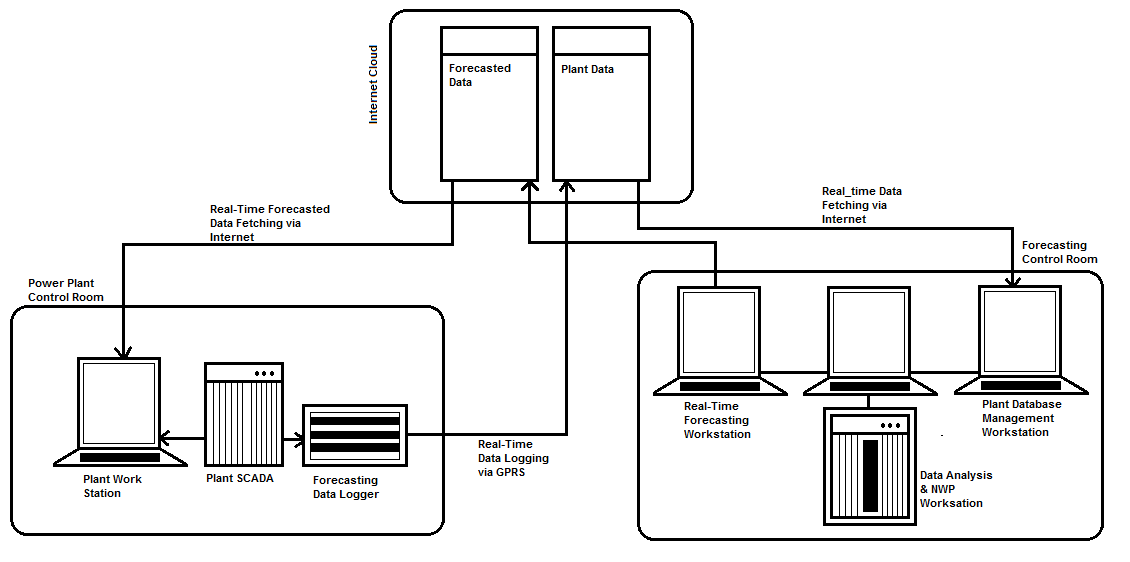
\includegraphics[scale=0.5]{ProposalDesign}
\caption{Future Work - Real-Time Forecasting System}
\label{figc10h1} %% to refer use, \ref{}
\end{figure}

The block diagram in Fig (\ref{figc10h1}) is explained as follows;\\

\begin{itemize}
  \item The Forecasting Data Logger is connected to the plant SCADA system, it sends real-time data to the plant data section of the internet cloud based server via GPRS; and it is independently powered, so as not to get affected by plant auxiliary power failure.
  \item The Plant Database Management Workstation hosts both the Forecasted Data and Plant Data servers on the internet cloud. It retrieves the plant data for real-time forecasting.
  \item The Real-Time Forecasting Workstation hosts the forecasting and energy estimation softwares which produce intra-hour, intra-day and day ahead forecasting reports for the respective plants and uploads it to the Forecasted Data server.
  \item The Data Analysis & NWP Workstation is used for big data analysis of the historical plant data for tuning the ARIMA and ANN forecasting models for respective plants. It also runs the NWP (Weather Research and Forecasting System) model for each plant site.
\end{itemize}

To summarize, the need for a forecasting mechanism for Renewable Energy generation plants is greater now than ever before. With foreign RE forecasting service providers dominating the market as there is no domestic alternative, we strive to develop an indigenous RE forecasting system which will be beneficial to the entire spectrum of the Indian Power Industry. The current status of work done forms a solid foundation, for scaling-up of the forecasting system to a form factor which will perform seamlessly in the field and be commercialized.\\